% Options for packages loaded elsewhere
\PassOptionsToPackage{unicode}{hyperref}
\PassOptionsToPackage{hyphens}{url}
%
\documentclass[
]{book}
\usepackage{amsmath,amssymb}
\usepackage{lmodern}
\usepackage{iftex}
\ifPDFTeX
  \usepackage[T1]{fontenc}
  \usepackage[utf8]{inputenc}
  \usepackage{textcomp} % provide euro and other symbols
\else % if luatex or xetex
  \usepackage{unicode-math}
  \defaultfontfeatures{Scale=MatchLowercase}
  \defaultfontfeatures[\rmfamily]{Ligatures=TeX,Scale=1}
\fi
% Use upquote if available, for straight quotes in verbatim environments
\IfFileExists{upquote.sty}{\usepackage{upquote}}{}
\IfFileExists{microtype.sty}{% use microtype if available
  \usepackage[]{microtype}
  \UseMicrotypeSet[protrusion]{basicmath} % disable protrusion for tt fonts
}{}
\makeatletter
\@ifundefined{KOMAClassName}{% if non-KOMA class
  \IfFileExists{parskip.sty}{%
    \usepackage{parskip}
  }{% else
    \setlength{\parindent}{0pt}
    \setlength{\parskip}{6pt plus 2pt minus 1pt}}
}{% if KOMA class
  \KOMAoptions{parskip=half}}
\makeatother
\usepackage{xcolor}
\usepackage{color}
\usepackage{fancyvrb}
\newcommand{\VerbBar}{|}
\newcommand{\VERB}{\Verb[commandchars=\\\{\}]}
\DefineVerbatimEnvironment{Highlighting}{Verbatim}{commandchars=\\\{\}}
% Add ',fontsize=\small' for more characters per line
\usepackage{framed}
\definecolor{shadecolor}{RGB}{248,248,248}
\newenvironment{Shaded}{\begin{snugshade}}{\end{snugshade}}
\newcommand{\AlertTok}[1]{\textcolor[rgb]{0.94,0.16,0.16}{#1}}
\newcommand{\AnnotationTok}[1]{\textcolor[rgb]{0.56,0.35,0.01}{\textbf{\textit{#1}}}}
\newcommand{\AttributeTok}[1]{\textcolor[rgb]{0.77,0.63,0.00}{#1}}
\newcommand{\BaseNTok}[1]{\textcolor[rgb]{0.00,0.00,0.81}{#1}}
\newcommand{\BuiltInTok}[1]{#1}
\newcommand{\CharTok}[1]{\textcolor[rgb]{0.31,0.60,0.02}{#1}}
\newcommand{\CommentTok}[1]{\textcolor[rgb]{0.56,0.35,0.01}{\textit{#1}}}
\newcommand{\CommentVarTok}[1]{\textcolor[rgb]{0.56,0.35,0.01}{\textbf{\textit{#1}}}}
\newcommand{\ConstantTok}[1]{\textcolor[rgb]{0.00,0.00,0.00}{#1}}
\newcommand{\ControlFlowTok}[1]{\textcolor[rgb]{0.13,0.29,0.53}{\textbf{#1}}}
\newcommand{\DataTypeTok}[1]{\textcolor[rgb]{0.13,0.29,0.53}{#1}}
\newcommand{\DecValTok}[1]{\textcolor[rgb]{0.00,0.00,0.81}{#1}}
\newcommand{\DocumentationTok}[1]{\textcolor[rgb]{0.56,0.35,0.01}{\textbf{\textit{#1}}}}
\newcommand{\ErrorTok}[1]{\textcolor[rgb]{0.64,0.00,0.00}{\textbf{#1}}}
\newcommand{\ExtensionTok}[1]{#1}
\newcommand{\FloatTok}[1]{\textcolor[rgb]{0.00,0.00,0.81}{#1}}
\newcommand{\FunctionTok}[1]{\textcolor[rgb]{0.00,0.00,0.00}{#1}}
\newcommand{\ImportTok}[1]{#1}
\newcommand{\InformationTok}[1]{\textcolor[rgb]{0.56,0.35,0.01}{\textbf{\textit{#1}}}}
\newcommand{\KeywordTok}[1]{\textcolor[rgb]{0.13,0.29,0.53}{\textbf{#1}}}
\newcommand{\NormalTok}[1]{#1}
\newcommand{\OperatorTok}[1]{\textcolor[rgb]{0.81,0.36,0.00}{\textbf{#1}}}
\newcommand{\OtherTok}[1]{\textcolor[rgb]{0.56,0.35,0.01}{#1}}
\newcommand{\PreprocessorTok}[1]{\textcolor[rgb]{0.56,0.35,0.01}{\textit{#1}}}
\newcommand{\RegionMarkerTok}[1]{#1}
\newcommand{\SpecialCharTok}[1]{\textcolor[rgb]{0.00,0.00,0.00}{#1}}
\newcommand{\SpecialStringTok}[1]{\textcolor[rgb]{0.31,0.60,0.02}{#1}}
\newcommand{\StringTok}[1]{\textcolor[rgb]{0.31,0.60,0.02}{#1}}
\newcommand{\VariableTok}[1]{\textcolor[rgb]{0.00,0.00,0.00}{#1}}
\newcommand{\VerbatimStringTok}[1]{\textcolor[rgb]{0.31,0.60,0.02}{#1}}
\newcommand{\WarningTok}[1]{\textcolor[rgb]{0.56,0.35,0.01}{\textbf{\textit{#1}}}}
\usepackage{longtable,booktabs,array}
\usepackage{calc} % for calculating minipage widths
% Correct order of tables after \paragraph or \subparagraph
\usepackage{etoolbox}
\makeatletter
\patchcmd\longtable{\par}{\if@noskipsec\mbox{}\fi\par}{}{}
\makeatother
% Allow footnotes in longtable head/foot
\IfFileExists{footnotehyper.sty}{\usepackage{footnotehyper}}{\usepackage{footnote}}
\makesavenoteenv{longtable}
\usepackage{graphicx}
\makeatletter
\def\maxwidth{\ifdim\Gin@nat@width>\linewidth\linewidth\else\Gin@nat@width\fi}
\def\maxheight{\ifdim\Gin@nat@height>\textheight\textheight\else\Gin@nat@height\fi}
\makeatother
% Scale images if necessary, so that they will not overflow the page
% margins by default, and it is still possible to overwrite the defaults
% using explicit options in \includegraphics[width, height, ...]{}
\setkeys{Gin}{width=\maxwidth,height=\maxheight,keepaspectratio}
% Set default figure placement to htbp
\makeatletter
\def\fps@figure{htbp}
\makeatother
\setlength{\emergencystretch}{3em} % prevent overfull lines
\providecommand{\tightlist}{%
  \setlength{\itemsep}{0pt}\setlength{\parskip}{0pt}}
\setcounter{secnumdepth}{5}
\usepackage{booktabs}
\ifLuaTeX
  \usepackage{selnolig}  % disable illegal ligatures
\fi
\usepackage[]{natbib}
\bibliographystyle{apalike}
\IfFileExists{bookmark.sty}{\usepackage{bookmark}}{\usepackage{hyperref}}
\IfFileExists{xurl.sty}{\usepackage{xurl}}{} % add URL line breaks if available
\urlstyle{same} % disable monospaced font for URLs
\hypersetup{
  pdftitle={Einführung in R},
  pdfauthor={Stephan Goerigk},
  hidelinks,
  pdfcreator={LaTeX via pandoc}}

\title{Einführung in R}
\author{Stephan Goerigk}
\date{2022-10-13}

\begin{document}
\maketitle

{
\setcounter{tocdepth}{1}
\tableofcontents
}
\hypertarget{uxfcber-dieses-skript}{%
\chapter*{Über dieses Skript}\label{uxfcber-dieses-skript}}
\addcontentsline{toc}{chapter}{Über dieses Skript}

Liebe Studierende,

dieses Skript soll Sie in die grundlegenden Analysewerkzeuge in R einführen, von der grundlegenden Kodierung und Analyse bis hin zur Datenverarbeitung, dem Plotten und der statistischen Inferenz.

Wenn R Ihre erste Programmiersprache ist, ist das völlig in Ordnung. Wir gehen alles Schritt für Schritt gemeinsam durch. Die Techniken in diesem Buch sind zwar auf die meisten Datenanalyseprobleme anwendbar, da wir jedoch aus der Psychologie kommen, werde ich den Kurs auf die Lösung von Analyseproblemen ausrichten, die in der psychologischen Forschung häufig auftreten.

\hypertarget{warum-ist-r-so-gut}{%
\chapter{Warum ist R so gut?}\label{warum-ist-r-so-gut}}

\hypertarget{open-source}{%
\section{Open Source}\label{open-source}}

R ist zu 100 \% kostenlos und verfügt daher über eine große Unterstützergemeinschaft. Im Gegensatz zu SPSS, Matlab, Excel und JMP ist R völlig kostenlos und wird es auch immer bleiben. Das hilft nicht nur Ihrem Geldbeutel - es bedeutet auch, dass eine riesige Gemeinschaft von R-Programmierern ständig neue R-Funktionen und -Pakete in einer Geschwindigkeit entwickelt und verbreitet, die alle anderen Pakete in den Schatten stellt. Die Größe der R-Programmiergemeinschaft ist atemberaubend. Wenn Sie jemals eine Frage dazu haben, wie man etwas in R implementiert, wird eine schnelle Google-Suche Sie praktisch jedes Mal zur Antwort führen.

\hypertarget{vielseitigkeit}{%
\section{Vielseitigkeit}\label{vielseitigkeit}}

R ist unglaublich vielseitig. Sie können R für alles verwenden, von der Berechnung einfacher zusammenfassender Statistiken über die Durchführung komplexer Simulationen bis hin zur Erstellung großartiger Diagramme. Wenn Sie sich eine analytische Aufgabe vorstellen können, können Sie sie mit ziemlicher Sicherheit in R implementieren.

\hypertarget{r-markdown}{%
\section{R Markdown}\label{r-markdown}}

Mit RStudio, einem Programm, das Sie beim Schreiben von R-Code unterstützt, können Sie mit RMarkdown einfach und nahtlos R-Code, Analysen, Diagramme und geschriebenen Text zu eleganten Dokumenten an einem Ort kombinieren. Tatsächlich habe ich dieses gesamte Skript (Text, Formatierung, Diagramme, Code\ldots{} ja, alles) in RStudio mit R Markdown geschrieben Mit RStudio müssen Sie sich nicht mehr mit zwei oder drei Programmen herumschlagen, z. B. Excel, Word und SPSS, wo Sie die Hälfte Ihrer Zeit mit dem Kopieren, Einfügen und Formatieren von Daten, Bildern und Tests verbringen, sondern können alles an einem Ort erledigen, so dass nichts mehr falsch gelesen, getippt oder vergessen wird.

\hypertarget{transparenz}{%
\section{Transparenz}\label{transparenz}}

In R durchgeführte Analysen sind transparent, leicht weiterzugeben und reproduzierbar. Wenn Sie einen SPSS-Benutzer fragen, wie er eine bestimmte Analyse durchgeführt hat, wird er sich ggf. nicht daran erinnern, was er vor Monaten oder Jahren tatsächlich getan hat. Wenn Sie einen R-Anwender (der gute Programmiertechniken verwendet) fragen, wie er eine Analyse durchgeführt hat, sollte er Ihnen immer den genauen Code zeigen können, den er verwendet hat. Das bedeutet natürlich nicht, dass er die richtige Analyse verwendet oder sie korrekt interpretiert hat, aber mit dem gesamten Originalcode sollten etwaige Probleme völlig transparent sein! Dies ist eine Grundvoraussetzung für offene, replizierbare Forschung.

\hypertarget{r-materialien}{%
\chapter{R Materialien}\label{r-materialien}}

\hypertarget{cheat-sheets}{%
\section{Cheat Sheets}\label{cheat-sheets}}

Im Laufe dieses Buches werden Sie viele neue Funktionen kennenlernen. Wäre es nicht schön, wenn jemand ein Wörterbuch mit vielen gängigen R-Funktionen erstellen würde? Ja, das wäre es, und zum Glück haben einige freundliche R-Programmierer genau das getan. Im Folgenden finden Sie eine Tabelle mit einigen der Funktionen, die ich empfehle. Ich empfehle Ihnen dringend, diese auszudrucken und die Funktionen zu markieren, wenn Sie sie lernen!

\href{https://cran.r-project.org/doc/contrib/Short-refcard.pdf}{Link zum Base R Cheat Sheet}

\href{https://www.rstudio.com/resources/cheatsheets/}{Link zu den R Studio Cheat Sheets}

Insbesondere die Cheat Sheets zu ggplot2 und dplyr kann ich Ihnen nur wärmstens ans Herz legen

\hypertarget{hilfe-und-inspiration-online}{%
\section{Hilfe und Inspiration online}\label{hilfe-und-inspiration-online}}

Eine Google Suche nach einem spezifischen R Problem bringt Sie (fast) immer an Ihr Ziel. Häufig findet man gute Antworten in den github Hilfsmatierialien einzelner Pakete, auf den Community Seiten von R Studio und in den Foren von stackoverflow.

\hypertarget{andere-buxfccher}{%
\section{Andere Bücher}\label{andere-buxfccher}}

Die Inhalte dieser Bücher sind nicht prüfunsrelevant.

Es gibt viele, viele ausgezeichnete Bücher über R. Hier sind zwei, die ich empfehlen kann (von denen eines sogar umsonst ist):

\href{https://www.amazon.com/Discovering-Statistics-Using-Andy-Field/dp/1446200469/ref=sr_1_2?ie=UTF8\&qid=1487759316\&sr=8-2\&keywords=statistics+with+r}{Discovering Statistics with R von Field, Miles and Field}

\href{http://r4ds.had.co.nz}{R for Data Science von Garrett Grolemund and Hadley Wickham}

\hypertarget{installation}{%
\chapter{Installation}\label{installation}}

Um R benutzen zu können müssen wir zwei Softwarepakete herunterladen:

\begin{itemize}
\tightlist
\item
  \textbf{R}
\item
  \textbf{RStudio}
\end{itemize}

R ist die Programmiersprache, mit der wir arbeiten. R-Studio ist eine Benutzeroberfläche, die uns das Programmieren mit R ungemein erleichtert.

\hypertarget{installation-von-r}{%
\section{Installation von R}\label{installation-von-r}}

Um R zu installieren, klicken Sie auf den, Ihrem Betriebssystem entsprechenden, Link und befolgen Sie die Anleitungen:

\begin{longtable}[]{@{}
  >{\raggedright\arraybackslash}p{(\columnwidth - 2\tabcolsep) * \real{0.5833}}
  >{\raggedright\arraybackslash}p{(\columnwidth - 2\tabcolsep) * \real{0.4167}}@{}}
\toprule()
\begin{minipage}[b]{\linewidth}\raggedright
Operating System
\end{minipage} & \begin{minipage}[b]{\linewidth}\raggedright
Link
\end{minipage} \\
\midrule()
\endhead
Windows & \url{http://cran.r-project.org/bin/windows/base/} \\
Mac & \url{http://cran.r-project.org/bin/macosx/} \\
\bottomrule()
\end{longtable}

Nach dieser Installation haben Sie bereits die volle Funktionalität des Programms. Sie werden jedoch feststellen, dass beinahe alle R-Nutzer RStudio zum programmieren nutzen, da dieses eine leichter nutzbare Oberfläche hat.
Tatsächlich müssen Sie nach der Installation von RStudio das R Basisprogramm nie wieder öffnen.

\hypertarget{installation-von-rstudio}{%
\section{Installation von RStudio}\label{installation-von-rstudio}}

Bitte installieren Sie dann RStudio - das Programm, über welches wir auf R zugreifen und mit dem wir unsere Skripte schreiben.

Um RStudio zu installieren, klicken Sie auf diesen Link und befolgen Sie die Anleitungen: \url{http://www.rstudio.com/products/rstudio/download/}

\hypertarget{programmaufbau}{%
\chapter{Programmaufbau}\label{programmaufbau}}

\hypertarget{die-vier-rstudio-fenster}{%
\section{Die vier RStudio Fenster}\label{die-vier-rstudio-fenster}}

Wenn Sie RStudio öffnen, sehen Sie vier Fenster, wie in der folgenden Abbildung dargestellt:

Wenn Sie mögen, können Sie die Reihenfolge der Fenster in den RStudio Einstellungen verändern.
Sie können die Fenster auch verstecken (Minimieren/Maximieren Symbol an der oberen rechten Ecke jedes Fensters) oder ihre Größe verändern, indem die sie ihre Grenzbalken anklicken und verschieben.

Lassen Sie uns jetzt schauen, was genau die Funktion jedes der Fenster ist:

\hypertarget{source---ihr-schreibblock-fuxfcr-code}{%
\subsection{Source - Ihr Schreibblock für Code}\label{source---ihr-schreibblock-fuxfcr-code}}

Im Source Fenster erstellen und bearbeiten Sie ``R-Skripte'' - Ihre Codesammlungen. Keine Sorge, R-Skripte sind nur Textdateien mit der Erweiterung ``.R''.
Wenn Sie RStudio öffnen, wird automatisch ein neues unbenanntes Skript gestartet.
Bevor Sie mit der Eingabe eines unbenannten R-Skripts beginnen, sollten Sie die Datei immer unter einem neuen Dateinamen speichern (z.B. ``Mein\_RScript.R'').
Wenn Ihr Computer während der Arbeit abstürzt, steht Ihr Code in R zur Verfügung, wenn Sie RStudio erneut öffnen.

Sie werden feststellen, dass R beim Schreiben des Skripts den Code während der Eingabe nicht tatsächlich ausführt. Damit R Ihren Code tatsächlich ausführt, müssen Sie den Code zunächst an die Konsole ``senden'' (wir werden im nächsten Abschnitt darüber sprechen).

Es gibt viele Möglichkeiten, Ihren Code aus dem Skript an die Konsole zu senden. Die langsamste Methode ist das Kopieren und Einfügen. Schneller geht es, wenn Sie den Code, den Sie auswerten möchten, markieren und auf die Schaltfläche ``Run'' oben rechts in der Quelle klicken. Alternativ können Sie auch die Tastenkombination ``Command + Return'' auf dem Mac oder ``Control + Enter'' auf dem PC verwenden, um den gesamten markierten Code an die Konsole zu senden.

\hypertarget{konsole---das-herzstuxfcck-von-r}{%
\subsection{Konsole - Das Herzstück von R}\label{konsole---das-herzstuxfcck-von-r}}

Die Konsole ist das Herzstück von R. Hier führt R den Code aus. Am Anfang der Konsole sehen Sie das Zeichen ``\textgreater{}''. Dies ist eine Eingabeaufforderung (sog. ``Prompt''), die Ihnen mitteilt, dass R bereit für neuen Code ist. Sie können direkt nach dem Prompt \texttt{\textgreater{}} Code in die Konsole eingeben und erhalten sofort eine Antwort. Wenn Sie zum Beispiel 2+2 in die Konsole eingeben und die Eingabetaste drücken, werden Sie sehen, dass R sofort eine Ausgabe von 4 liefert.

\begin{Shaded}
\begin{Highlighting}[]
\DecValTok{2}\SpecialCharTok{+}\DecValTok{2}
\end{Highlighting}
\end{Shaded}

\begin{verbatim}
## [1] 4
\end{verbatim}

Versuchen Sie, 2+2 zu berechnen, indem Sie den Code direkt in die Konsole eingeben - und dann Enter drücken.
Sie sollten das Ergebnis \texttt{{[}1{]}\ 4} sehen. Machen Sie sich keine Gedanken über die \texttt{{[}1{]}}, dazu kommen wir später.

Geben Sie denselben Code in das Skript ein und senden Sie ihn an die Konsole, indem Sie den Code markieren und auf die Schaltfläche ``Run'' in der oberen rechten Ecke des Quelltextfensters klicken. Alternativ können Sie auch die Tastenkombination ``Command + Return'' auf dem Mac oder ``Control + Enter'' unter Windows verwenden.

\textbf{Tipp}: Wie Sie sehen, können Sie Code entweder über das Skript oder durch direkte Eingabe in die Konsole ausführen. In 99\% der Fälle sollten Sie jedoch das Skript und nicht die Konsole verwenden. Der Grund dafür ist ganz einfach: Wenn Sie den Code in die Konsole eingeben, wird er nicht gespeichert (obwohl Sie in Ihrem Befehlsverlauf nachsehen können). Und wenn Sie beim Eingeben von Code in die Konsole einen Fehler machen, müssen Sie alles noch einmal von vorne eingeben. Stattdessen ist es besser, den gesamten Code in das Skript zu schreiben. Wenn Sie bereit sind, einen Code auszuführen, können Sie ihn mit ``Run'' an die Konsole senden.

\hypertarget{environmenthistory---das-geduxe4chtnis-von-r}{%
\subsection{Environment/History - Das Gedächtnis von R}\label{environmenthistory---das-geduxe4chtnis-von-r}}

In dem Tab ``Environtment'' dieses Bereichs werden die Namen aller Datenobjekte (wie Vektoren, Matrizen und Datenrahmen) angezeigt, die Sie in Ihrer aktuellen R-Session definiert haben. Sie können auch Informationen wie die Anzahl der Spalten und Zeilen in Datensätzen sehen. Der Tab enthält auch einige anklickbare Aktionen wie\\
Datensatz importieren'', wodurch eine grafische Benutzeroberfläche (GUI) für wichtige Daten in R geöffnet wird.

Der Tab ``Historiy'' dieses Bereichs zeigt Ihnen einfach eine Sammlung aller Befehle an den Sie zuvor in der Konsole ausgewertet haben. Wenn man mit Skripten arbeitet, schaut man sich diese, allerdings relativ selten an.

Wenn Sie sich mit R besser auskennen, werden Sie das Fenster Environment/History vielleicht nützlich finden. Aber für den Moment können Sie es einfach ignorieren. Wenn Sie Ihren Bildschirm entrümpeln wollen, können Sie das Fenster auch einfach minimieren, indem Sie auf die Schaltfläche Minimieren oben rechts im Fenster klicken.

\hypertarget{filesplotspackageshelpviewer---interaktion-von-r-mit-dateien}{%
\subsection{Files/Plots/Packages/Help/Viewer - Interaktion von R mit Dateien}\label{filesplotspackageshelpviewer---interaktion-von-r-mit-dateien}}

Die Tabs Files/Plots/Packages/Help/Viewer zeigen Ihnen viele hilfreiche Informationen. Schauen wir uns die einzelnen Registerkarten im Detail an:

\begin{enumerate}
\def\labelenumi{\arabic{enumi}.}
\item
  Files - Der Tab ``Files'' gibt Ihnen Zugriff auf das Dateiverzeichnis auf Ihrer Festplatte. Dateien, die Sie in Ihrem R Projekt benutzen liegen in der Regel in einem von Ihnen definierten Arbeitsverzeichnis. Wir werden in Kürze ausführlicher über Arbeitsverzeichnisse sprechen.
\item
  Plots - Das Plots-Panel zeigt (keine große Überraschung) alle Ihre Plots an.
\item
  Pakete - Zeigt eine Liste aller auf Ihrer Festplatte installierten R-Pakete an und gibt an, ob sie derzeit geladen sind oder nicht. Pakete, die in der aktuellen Sitzung geladen sind, sind markiert, während Pakete, die installiert, aber noch nicht geladen sind, nicht markiert sind. Auf die Pakete gehen wir im nächsten Abschnitt näher ein.
\item
  Hilfe - Hilfemenü für R-Funktionen. Sie können entweder den Namen einer Funktion in das Suchfenster eingeben oder den Code \texttt{?function.name} verwenden, um nach einer Funktion mit dem Namen \texttt{function.name} zu suchen:
\end{enumerate}

\begin{Shaded}
\begin{Highlighting}[]
\NormalTok{?hist   }\CommentTok{\# Wie funktioniert die Histogrammfunktion?}
\NormalTok{?t.test }\CommentTok{\# Wie funktioniert der t{-}Test?}
\end{Highlighting}
\end{Shaded}

\hypertarget{r-packages}{%
\section{R Packages}\label{r-packages}}

Wenn Sie R zum ersten Mal herunterladen und installieren, installieren Sie die Base R Software.
Base R enthält die meisten Funktionen, die Sie täglich verwenden werden, wie mean() und hist().
Allerdings werden hier nur Funktionen angezeigt, die von den ursprünglichen Autoren der Sprache R geschrieben wurden.
Wenn Sie auf Daten und Code zugreifen möchten, die von anderen Personen geschrieben wurden, müssen Sie diese als ``Package'' installieren.
Ein R-Package ist einfach ein Bündel von Funktionen (also bereits geschriebener Code), die in einem übersichtlichen Paket gespeichert sind.

Ein Paket ist wie eine Glühbirne. Um es nutzen zu können, müssen Sie es zunächst in Ihr Haus (d.h. auf Ihren Computer) bestellen, indem Sie es installieren. Wenn Sie ein Paket einmal installiert haben, brauchen Sie es nie wieder zu installieren. Jedes Mal, wenn Sie das Paket tatsächlich verwenden wollen, müssen Sie es jedoch einschalten, indem Sie es laden. Und so geht's:

\hypertarget{r-packages-installieren}{%
\subsection{R Packages installieren}\label{r-packages-installieren}}

Ein Paket zu installieren bedeutet einfach, den Paketcode auf Ihren Computer herunterzuladen. Die gängigste Methode ist das Herunterladen aus dem Comprehensive R Archive Network (CRAN).

Um ein neues R-Paket von CRAN zu installieren, können Sie einfach den Code install.packages(``name'') ausführen, wobei ``name'' der Name des Pakets ist.

Um zum Beispiel das Paket ggplot2 herunterzuladen, welches wir oft zum Erstellen von Graphen verwenden, geben Sie ein:

\begin{Shaded}
\begin{Highlighting}[]
\CommentTok{\# install.packages("ggplot2")}
\end{Highlighting}
\end{Shaded}

\hypertarget{r-packages-laden}{%
\subsection{R Packages laden}\label{r-packages-laden}}

Sobald Sie ein Paket installiert haben, befindet es sich auf Ihrem Computer. Aber nur weil es auf Ihrem Computer ist, bedeutet das nicht, dass R bereit ist, es zu benutzen. Wenn Sie etwas, wie eine Funktion oder einen Datensatz, aus einem Paket verwenden wollen, müssen Sie \emph{immer} zuerst das Paket in Ihrer R-Sitzung \emph{laden}. Genau wie bei einer Glühbirne müssen Sie sie einschalten, um sie zu benutzen!

Um ein Paket zu laden, verwenden Sie die Funktion \texttt{library()}. Nachdem wir zum Beispiel das Paket \texttt{ggplot2} installiert haben, können wir es mit \texttt{library("ggplot2")} laden:

\begin{Shaded}
\begin{Highlighting}[]
\CommentTok{\#   Laden des "ggplot2" Pakekts, damit wir es benutzen können!}
\CommentTok{\#   Pakete müssen zu Beginn jeder R Session neu geladen werden!}
\FunctionTok{library}\NormalTok{(}\StringTok{"ggplot2"}\NormalTok{)}
\end{Highlighting}
\end{Shaded}

Jetzt, wo Sie das Paket \texttt{ggplot2} geladen haben, können Sie jede seiner Funktionen benutzen (hier die Funktion ggplot, um einen Graph zu erstellen)!

\begin{Shaded}
\begin{Highlighting}[]
\FunctionTok{ggplot}\NormalTok{(}\AttributeTok{data =}\NormalTok{ iris, }\FunctionTok{aes}\NormalTok{(}\AttributeTok{x =}\NormalTok{ Sepal.Length)) }\SpecialCharTok{+} 
  \FunctionTok{geom\_histogram}\NormalTok{()}
\end{Highlighting}
\end{Shaded}

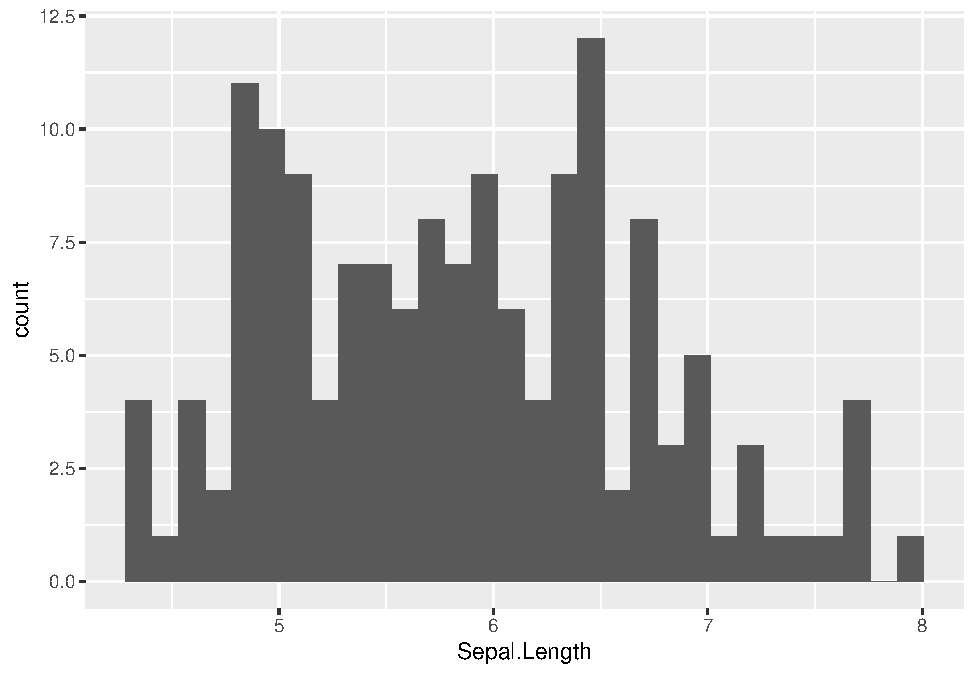
\includegraphics{CFH_R_bookdown_files/figure-latex/unnamed-chunk-6-1.pdf}

Pakete müssen zu Beginn jeder R Session neu geladen werden. Deswegen schreiben wir in der Regel ganz an den Anfang unseres Skripts gleich mehrere Zeilen, mit \texttt{library()} Befehlen für alle R Pakete, die wir für unsere Analyse benötigen werden.

In R gibt es eine Möglichkeit, ein Paket vorübergehend zu laden, ohne die Funktion \texttt{library()} zu verwenden. Um dies zu tun, können Sie einfach die Notation \texttt{package::funktion} verwenden. Diese Notation sagt R einfach, dass es das Paket nur für diesen einen Codeabschnitt laden soll. Zum Beispiel könnte ich die Funktion \texttt{ggplot} aus dem Paket \texttt{ggplot2} wie folgt verwenden:

\begin{Shaded}
\begin{Highlighting}[]
\NormalTok{ggplot2}\SpecialCharTok{::}\FunctionTok{ggplot}\NormalTok{(}\AttributeTok{data =}\NormalTok{ iris, }\FunctionTok{aes}\NormalTok{(}\AttributeTok{x =}\NormalTok{ Sepal.Length)) }\SpecialCharTok{+} 
  \FunctionTok{geom\_histogram}\NormalTok{()}
\end{Highlighting}
\end{Shaded}

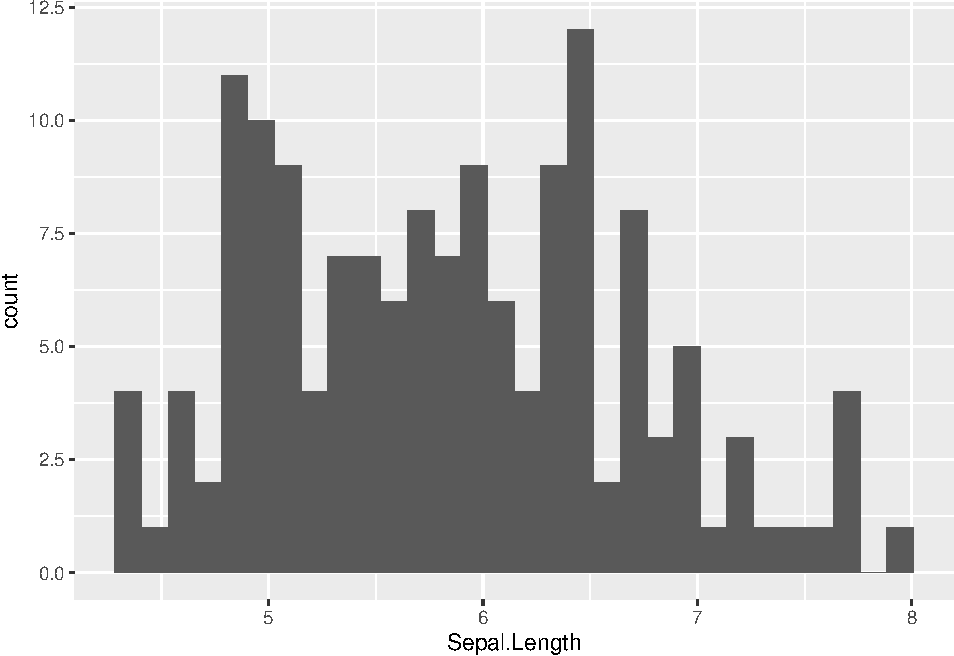
\includegraphics{CFH_R_bookdown_files/figure-latex/unnamed-chunk-7-1.pdf}

Ein Vorteil der Notation ``package::function'' ist, dass für jeden, der den Code liest, sofort klar ist, welches Paket die Funktion enthält. Ein Nachteil ist jedoch, dass Sie, wenn Sie eine Funktion aus einem Paket häufig verwenden, gezwungen sind, den Paketnamen ständig neu einzugeben. Sie können jede Methode verwenden, die für Sie sinnvoll ist.

\hypertarget{datenformate}{%
\chapter{Datenformate}\label{datenformate}}

\begin{figure}
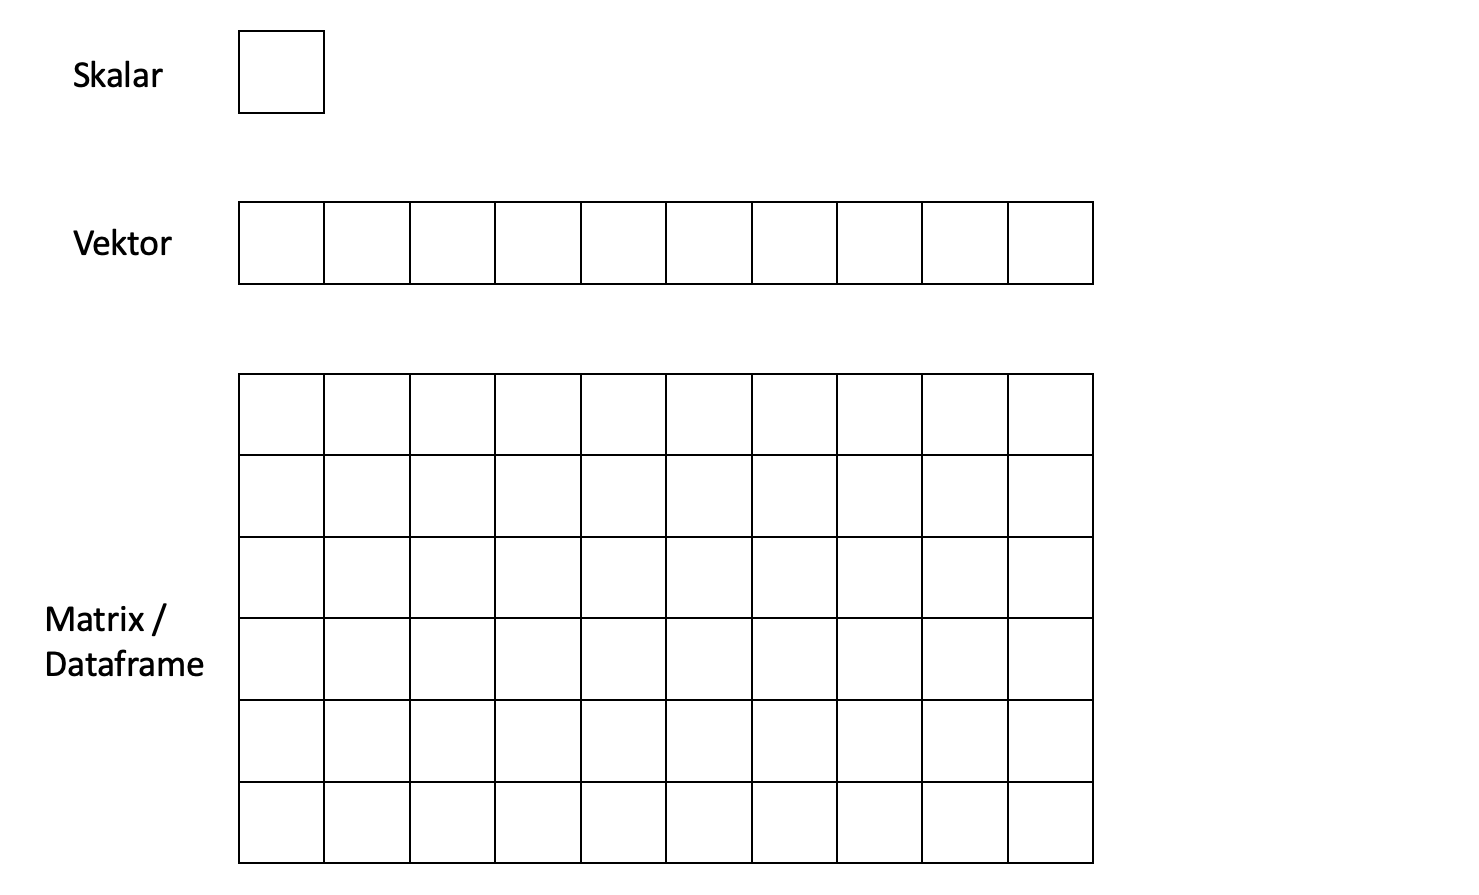
\includegraphics[width=20.54in]{images/Datenformat_1} \caption{Skalar, Vektor, Matrix}\label{fig:unnamed-chunk-8}
\end{figure}

\hypertarget{skalar}{%
\section{Skalar}\label{skalar}}

Der einfachste Objekttyp in R ist der \textbf{Skalar}. Ein Skalar Objekt ist einfach nur ein einzelner Wert, z.B. eine Zahl oder ein Wort.

Hier sind einige Beispiele für numerische Skalar Objekte:

\begin{Shaded}
\begin{Highlighting}[]
\CommentTok{\# Examples of numeric scalars}
\NormalTok{a }\OtherTok{\textless{}{-}} \DecValTok{100}
\NormalTok{b }\OtherTok{\textless{}{-}} \DecValTok{3} \SpecialCharTok{/} \DecValTok{100}
\NormalTok{c }\OtherTok{\textless{}{-}}\NormalTok{ (a }\SpecialCharTok{+}\NormalTok{ b) }\SpecialCharTok{/}\NormalTok{ b}
\end{Highlighting}
\end{Shaded}

Skalare müssen nicht numerisch sein, sondern auch Worte. Wortobjekte heißen in R \textbf{characters} (aka strings). In R schreibt man characters immer in Anführungszeichen \texttt{""}. Hier sind einige Beispiele für character Skalare:

\begin{Shaded}
\begin{Highlighting}[]
\CommentTok{\# Beispiele für character Skalare}
\NormalTok{d }\OtherTok{\textless{}{-}} \StringTok{"Psychologe"}
\NormalTok{e }\OtherTok{\textless{}{-}} \StringTok{"Zigarre"}
\NormalTok{f }\OtherTok{\textless{}{-}} \StringTok{"Haben Psychologen wirklich alle Bärte und rauchen Zigarre?"}
\end{Highlighting}
\end{Shaded}

Wie Sie sich vermutlich vorstellen können, behandelt R numerische und character Skalare unterschiedlich. Zum Beispiel lassen sich mir numerischen Skalaren grundlegende arithmetische Operationen durchfühlen (Addition, Subtraktion, Multiplikation\ldots) -- das funktioniert mit character Skalaren nicht.
Wenn Sie dennoch probieren numerische Operationen auf character Skalare anzuwenden, bekommen Sie eine Fehlermeldung, so wie diese:

\begin{Shaded}
\begin{Highlighting}[]
\NormalTok{a }\OtherTok{=} \StringTok{"1"}
\NormalTok{b }\OtherTok{=} \StringTok{"2"}
\NormalTok{a }\SpecialCharTok{+}\NormalTok{ b}
\end{Highlighting}
\end{Shaded}

\emph{``Fehler in a + b : nicht-numerisches Argument für binären Operator''}

\hypertarget{vektor}{%
\section{Vektor}\label{vektor}}

Machen wir weiter mit \texttt{Vektoren}. Ein Vektor Objekt ist einfach eine Kombination mehrerer Skalare in einem einzelnen Objekt (z.B. eine Zahlen- oder Wortreihe).
Zum Beispiel könnten die Zahlen von 1-10 in einen Vektor mit der Länge 10 kombiniert werden. Oder die Buchstaben des Alphabets könnten in einen Vektor mit der Länge 26 gespeichert werden. Genau wie Skalare, können Vektoren numerisch oder characters sein (Aber nicht beides auf einmal!)

Die einfachste Art einen Vektor zu erstellen ist mit der \texttt{c()} Funktion. Das c steht für ``concatenate'', was auf Englisch so viel heißt wie ``zusammenbringen''. Die \texttt{c()} Funktion nimmt mehrere Skalare als Input und erstellt einen Vektor, der diese Objekte enthält.

Wenn man\texttt{c()} benutzt, muss man immer ein \textbf{Komma} zwischen die Objekte setzen (Skalare oder Vektoren), die man kombinieren möchte.

Lassen Sie uns die \texttt{c()} Funktion nutzen um einen Vektor zu erstellen der \texttt{a} heißt und die Zahlen von 1 bis 7 enthält

Let's use the \texttt{c()} function to create a vector called \texttt{a} containing the integers from 1 to 5.

\begin{Shaded}
\begin{Highlighting}[]
\NormalTok{a }\OtherTok{=} \FunctionTok{c}\NormalTok{(}\DecValTok{1}\NormalTok{, }\DecValTok{2}\NormalTok{, }\DecValTok{3}\NormalTok{, }\DecValTok{4}\NormalTok{, }\DecValTok{5}\NormalTok{, }\DecValTok{6}\NormalTok{, }\DecValTok{7}\NormalTok{)}
\CommentTok{\# Das Ergebnis ausgeben}
\NormalTok{a}
\end{Highlighting}
\end{Shaded}

\begin{verbatim}
## [1] 1 2 3 4 5 6 7
\end{verbatim}

Sie können auch character Vektoren erstellen, indem Sie die \texttt{c()} auf einzelne character Skalare Funktion anwenden:

\begin{Shaded}
\begin{Highlighting}[]
\NormalTok{char.vec }\OtherTok{=} \FunctionTok{c}\NormalTok{(}\StringTok{"Freud"}\NormalTok{, }\StringTok{"Wundt"}\NormalTok{, }\StringTok{"Bandura"}\NormalTok{, }\StringTok{"Watson"}\NormalTok{, }\StringTok{"Jung"}\NormalTok{)}
\CommentTok{\# Das Ergebnis ausgeben}
\NormalTok{char.vec}
\end{Highlighting}
\end{Shaded}

\begin{verbatim}
## [1] "Freud"   "Wundt"   "Bandura" "Watson"  "Jung"
\end{verbatim}

\hypertarget{vektor-typen}{%
\subsection{Vektor Typen}\label{vektor-typen}}

Vektoren sind ein zentrales Element von R. Ein Vektor kann Zahlen, Buchstaben oder logische Werte enthalten, aber niemals eine Kombination

Der Vektor ist die Entsprechung der \textbf{Variable} und die Skalare, aus denen der Vektor besteht sind die \textbf{Merkmalsausprägungen} der Variable.

\hypertarget{faktor-variablen}{%
\subsection{Faktor Variablen}\label{faktor-variablen}}

Wir haben bereits gelernt, wie man einen Vektor aus character Objekten erstellt. Manchmal brauchen wir in R jedoch Variablen, die nicht nur Worte enthalten, sondern dem Programm mitteilen, dass es sich um feste Gruppen oder \textbf{Kategorien} handelt. Es geht also nicht nur um eine ``Sammlung'' von Worten (z.B. Nachnamen von Probanden), sondern um festgelegte Analyseeinheiten. Solche Variablen heißen in R \texttt{factor}.

In einer factor Variable ist jeder Kategorie eine Zahl zugeordnet (z.B. 1 = männlich, 2 = weiblich).

Um Faktor Variablen zu erstellen, machen wie einen Vorgang, den man \textbf{Kodieren} nennt und das geht so:

Wir haben einen Vektor mit Codes 1 und 2 für männlich und weiblich vorliegen:

\begin{Shaded}
\begin{Highlighting}[]
\NormalTok{geschlecht }\OtherTok{=} \FunctionTok{c}\NormalTok{(}\DecValTok{1}\NormalTok{, }\DecValTok{2}\NormalTok{, }\DecValTok{2}\NormalTok{, }\DecValTok{1}\NormalTok{, }\DecValTok{2}\NormalTok{)}
\CommentTok{\# Das Ergebnis ausgeben}
\NormalTok{geschlecht}
\end{Highlighting}
\end{Shaded}

\begin{verbatim}
## [1] 1 2 2 1 2
\end{verbatim}

In dieser Form erkennt R diesen Vektor als numerische Variable. Um Sie in einen Faktor umzuwandeln, definieren wir die Zahlen (1 und 2) als \texttt{levels} des Faktors und geben dann jedem level einen Namen (\texttt{labels}):

\begin{Shaded}
\begin{Highlighting}[]
\NormalTok{geschlecht }\OtherTok{=} \FunctionTok{factor}\NormalTok{(geschlecht, }\AttributeTok{levels =} \FunctionTok{c}\NormalTok{(}\DecValTok{1}\NormalTok{,}\DecValTok{2}\NormalTok{), }\AttributeTok{labels =} \FunctionTok{c}\NormalTok{(}\StringTok{"männlich"}\NormalTok{, }\StringTok{"weiblich"}\NormalTok{))}
\CommentTok{\# Das Ergebnis ausgeben}
\NormalTok{geschlecht}
\end{Highlighting}
\end{Shaded}

\begin{verbatim}
## [1] männlich weiblich weiblich männlich weiblich
## Levels: männlich weiblich
\end{verbatim}

Das Ergebnis ist eine codierte Faktorvariable. Wenn wir Sie uns ausgeben lassen erhalten wir unter den Merkmalsausprägungen eine Liste mit den einzelnen Kategorien (levels) des Faktors.

R wird uns für Faktoren alle Ergebnisse nach der \textbf{Reihenfolge} der levels anzeigen. Wenn wir keine Faktorvariable haben, sondern eine character Variable funktioniert die Reihenfolge immer alphabetisch.

\hypertarget{vektor-indizierung}{%
\subsection{Vektor Indizierung}\label{vektor-indizierung}}

Manchmal möchten wir wieder einen einzelnen Skalar auswählen, der als Teil von einem Vektor gespeichert ist. Diese \textbf{Auswahl} eines Einzelelements nennt man \textbf{Indizierung}. Die Auswahl eines kleineren Objekts aus einem größeren Objekt funktioniert in R immer mit \texttt{{[}{]}}.

Benötigen wir aus einem Vektor z.B. genau den 3. Skalar, schreiben wir einfach eine 3 in eckige Klammern hinter den Vektor.

\begin{Shaded}
\begin{Highlighting}[]
\NormalTok{char.vec }\OtherTok{=} \FunctionTok{c}\NormalTok{(}\StringTok{"Freud"}\NormalTok{, }\StringTok{"Wundt"}\NormalTok{, }\StringTok{"Bandura"}\NormalTok{, }\StringTok{"Watson"}\NormalTok{, }\StringTok{"Jung"}\NormalTok{)}
\CommentTok{\# Das Ergebnis ausgeben}
\NormalTok{char.vec[}\DecValTok{5}\NormalTok{]}
\end{Highlighting}
\end{Shaded}

\begin{verbatim}
## [1] "Jung"
\end{verbatim}

\hypertarget{matrizen-und-dataframes}{%
\section{Matrizen und Dataframes}\label{matrizen-und-dataframes}}

In der Psychologie beobachten wir für unsere Studien fast immer mehr als eine Variable. Wir könnten diese alle in einzelnen Vektoren speichern und uns die Objektnamen merken. Z.B.

\begin{Shaded}
\begin{Highlighting}[]
\NormalTok{Name }\OtherTok{=} \FunctionTok{c}\NormalTok{(}\StringTok{"Max"}\NormalTok{, }\StringTok{"Maja"}\NormalTok{, }\StringTok{"Mia"}\NormalTok{, }\StringTok{"Moritz"}\NormalTok{, }\StringTok{"Markus"}\NormalTok{)}
\NormalTok{Alter }\OtherTok{=} \FunctionTok{c}\NormalTok{(}\DecValTok{20}\NormalTok{, }\DecValTok{31}\NormalTok{, }\DecValTok{25}\NormalTok{, }\DecValTok{34}\NormalTok{, }\DecValTok{51}\NormalTok{)}
\NormalTok{Diagnose }\OtherTok{=} \FunctionTok{c}\NormalTok{(}\StringTok{"Depression"}\NormalTok{, }\StringTok{"Zwangsstörung"}\NormalTok{, }\StringTok{"Depression"}\NormalTok{, }\StringTok{"Soziale Phobie"}\NormalTok{, }\StringTok{"Depression"}\NormalTok{)}
\end{Highlighting}
\end{Shaded}

\hypertarget{erstellen-von-datenmatrizen}{%
\subsection{Erstellen von Datenmatrizen}\label{erstellen-von-datenmatrizen}}

Praktischer ist es, die einzelnen Vektoren in Tabellenform zu speichern, der \textbf{Datenmatrix}. In R heißen Datenmatrizen \texttt{data.frame}. Wir können die Vektoren folgendermaßen zu einem data.frame kombinieren:

\begin{Shaded}
\begin{Highlighting}[]
\NormalTok{df }\OtherTok{=} \FunctionTok{data.frame}\NormalTok{(Name, Alter, Diagnose)}
\CommentTok{\# Das Ergebnis ausgeben}
\NormalTok{df}
\end{Highlighting}
\end{Shaded}

\begin{verbatim}
##     Name Alter       Diagnose
## 1    Max    20     Depression
## 2   Maja    31  Zwangsstörung
## 3    Mia    25     Depression
## 4 Moritz    34 Soziale Phobie
## 5 Markus    51     Depression
\end{verbatim}

Wie in jeder Datenmatrix entsprechen die \textbf{Zeilen} den einzelnen Personen (Fällen) und die \textbf{Spalten} den Variablen.

R bezeichnet Zeilen und Spalten als \textbf{rows} und \textbf{columns}. Wollen wir z.B. wissen, wie viele Zeilen der data.frame hat, können wir \texttt{nrow()} benutzen. Für die Anzahl der Spalten nehmen wir \texttt{ncol()}:

\begin{Shaded}
\begin{Highlighting}[]
\FunctionTok{nrow}\NormalTok{(df)}
\end{Highlighting}
\end{Shaded}

\begin{verbatim}
## [1] 5
\end{verbatim}

\begin{Shaded}
\begin{Highlighting}[]
\FunctionTok{ncol}\NormalTok{(df)}
\end{Highlighting}
\end{Shaded}

\begin{verbatim}
## [1] 3
\end{verbatim}

Wenn wir die einzelnen Vektoren nicht bereits vorher definiert haben, können wir auch alles in einem Schritt machen. Das Ergebnis ist das gleiche:

\begin{Shaded}
\begin{Highlighting}[]
\NormalTok{df }\OtherTok{=} \FunctionTok{data.frame}\NormalTok{(}\StringTok{"Name"} \OtherTok{=} \FunctionTok{c}\NormalTok{(}\StringTok{"Max"}\NormalTok{, }\StringTok{"Maja"}\NormalTok{, }\StringTok{"Mia"}\NormalTok{, }\StringTok{"Moritz"}\NormalTok{, }\StringTok{"Markus"}\NormalTok{),}
                \StringTok{"Alter"} \OtherTok{=} \FunctionTok{c}\NormalTok{(}\DecValTok{20}\NormalTok{, }\DecValTok{31}\NormalTok{, }\DecValTok{25}\NormalTok{, }\DecValTok{34}\NormalTok{, }\DecValTok{51}\NormalTok{),}
                \StringTok{"Diagnose"} \OtherTok{=} \FunctionTok{c}\NormalTok{(}\StringTok{"Depression"}\NormalTok{, }\StringTok{"Zwangsstörung"}\NormalTok{, }\StringTok{"Depression"}\NormalTok{, }\StringTok{"Soziale Phobie"}\NormalTok{, }\StringTok{"Depression"}\NormalTok{)}
\NormalTok{                )}
\CommentTok{\# Das Ergebnis ausgeben}
\NormalTok{df}
\end{Highlighting}
\end{Shaded}

\begin{verbatim}
##     Name Alter       Diagnose
## 1    Max    20     Depression
## 2   Maja    31  Zwangsstörung
## 3    Mia    25     Depression
## 4 Moritz    34 Soziale Phobie
## 5 Markus    51     Depression
\end{verbatim}

Wollen wir wieder eine einzelne Variable aus dem benutzen, können wir diese über das \texttt{\$} Zeichen anwählen:

\begin{Shaded}
\begin{Highlighting}[]
\NormalTok{df}\SpecialCharTok{$}\NormalTok{Alter}
\end{Highlighting}
\end{Shaded}

\begin{verbatim}
## [1] 20 31 25 34 51
\end{verbatim}

\hypertarget{indizierung}{%
\subsection{Indizierung}\label{indizierung}}

Wollen wir aus dem data.frame wieder einzelne Elemente benutzen, nutzen wir wieder die Indizierung. Auch hier brauchen wir die \texttt{{[}{]}}. Da wir im data.frame Zeilen und Spalten haben, brauchen wir eine Möglichkeit beides auszuwählen, wie ein Curser der von links nach rechts, bzw. von oben nach unten läuft.

Wir trennen dafür unsere \texttt{{[}{]}} mit einem Komma \texttt{{[},{]}}. Alles was \textbf{links vom Komma} steht bezieht sich auf Zeilen alles \textbf{rechts vom Komma} bezieht sich auf Spalten.

Lassen Sie uns einmal die Zelle in der 1. Zeile (also die 1. Person) und der 3. Variable auswählen:

\begin{Shaded}
\begin{Highlighting}[]
\NormalTok{df[}\DecValTok{1}\NormalTok{,}\DecValTok{3}\NormalTok{]}
\end{Highlighting}
\end{Shaded}

\begin{verbatim}
## [1] Depression
## Levels: Depression Soziale Phobie Zwangsstörung
\end{verbatim}

Lassen wir die Zahl vor dem Komma weg, bekommen wir alle Werte aus der Spalte:

\begin{Shaded}
\begin{Highlighting}[]
\NormalTok{df[,}\DecValTok{3}\NormalTok{]}
\end{Highlighting}
\end{Shaded}

\begin{verbatim}
## [1] Depression     Zwangsstörung  Depression     Soziale Phobie Depression    
## Levels: Depression Soziale Phobie Zwangsstörung
\end{verbatim}

Lassen wir die Zahl nach dem Komma weg, bekommen wir alle Werte aus der Reihe:

\begin{Shaded}
\begin{Highlighting}[]
\NormalTok{df[}\DecValTok{1}\NormalTok{,]}
\end{Highlighting}
\end{Shaded}

\begin{verbatim}
##   Name Alter   Diagnose
## 1  Max    20 Depression
\end{verbatim}

\hypertarget{daten-erstellen}{%
\chapter{Daten erstellen}\label{daten-erstellen}}

\hypertarget{manuell}{%
\section{Manuell}\label{manuell}}

Die manuelle Eingabe von Daten erfolgt über die \texttt{c()} Funktion. Mit ihrer Hilfe können wir Skalare zu Vektoren verbinden\ldots{}

\begin{Shaded}
\begin{Highlighting}[]
\NormalTok{a }\OtherTok{=} \FunctionTok{c}\NormalTok{(}\DecValTok{1}\NormalTok{, }\DecValTok{2}\NormalTok{, }\DecValTok{4}\NormalTok{, }\DecValTok{6}\NormalTok{, }\DecValTok{1}\NormalTok{)}
\end{Highlighting}
\end{Shaded}

\ldots mehrere Vektoren aneinanderhängen\ldots{}

\begin{Shaded}
\begin{Highlighting}[]
\NormalTok{a }\OtherTok{=} \FunctionTok{c}\NormalTok{(}\DecValTok{1}\NormalTok{, }\DecValTok{2}\NormalTok{, }\DecValTok{4}\NormalTok{, }\DecValTok{6}\NormalTok{, }\DecValTok{1}\NormalTok{)}
\NormalTok{b }\OtherTok{=} \FunctionTok{c}\NormalTok{(}\DecValTok{2}\NormalTok{, }\DecValTok{3}\NormalTok{)}
\NormalTok{c }\OtherTok{=} \FunctionTok{c}\NormalTok{(a, b)}
\NormalTok{c}
\end{Highlighting}
\end{Shaded}

\begin{verbatim}
## [1] 1 2 4 6 1 2 3
\end{verbatim}

\ldots und Vektoren gleicher Länge zu data.frames kombinieren:

\begin{Shaded}
\begin{Highlighting}[]
\NormalTok{daten }\OtherTok{=} \FunctionTok{data.frame}\NormalTok{(}\AttributeTok{aufmerksamkeit =} \FunctionTok{c}\NormalTok{(}\DecValTok{58}\NormalTok{, }\DecValTok{46}\NormalTok{, }\DecValTok{29}\NormalTok{, }\DecValTok{51}\NormalTok{),}
                   \AttributeTok{gedaechtnis =} \FunctionTok{c}\NormalTok{(}\DecValTok{22}\NormalTok{, }\DecValTok{67}\NormalTok{, }\DecValTok{22}\NormalTok{, }\DecValTok{31}\NormalTok{))}
\NormalTok{daten}
\end{Highlighting}
\end{Shaded}

\begin{verbatim}
##   aufmerksamkeit gedaechtnis
## 1             58          22
## 2             46          67
## 3             29          22
## 4             51          31
\end{verbatim}

\hypertarget{automatisch}{%
\section{Automatisch}\label{automatisch}}

Wir haben bereits die \texttt{c()} Funktion gelernt.

Die \texttt{c()} Funktion ist die einfachste Art einen Vektor zu erstellen, sie ist aber vermutlich auch die umständlichste. Stellen Sie sich zum Beispiel vor, Sie wollen einen Vektor erstellen, der alle Zahlen von 0 bis 100 enthält. Diese Zahlen wollen Sie definitiv nicht alle in die Klammer von \texttt{c()} eintippen.

Glücklicherweise hat R viele eingebaute Funktionen, um leicht automatisch numerische Vektoren zu erstellen.

Lassen Sie uns mit dreien davon starten\texttt{a:b}, \texttt{seq()}, and \texttt{rep()}:

\begin{longtable}[]{@{}
  >{\raggedright\arraybackslash}p{(\columnwidth - 4\tabcolsep) * \real{0.3881}}
  >{\raggedright\arraybackslash}p{(\columnwidth - 4\tabcolsep) * \real{0.4478}}
  >{\raggedright\arraybackslash}p{(\columnwidth - 4\tabcolsep) * \real{0.1642}}@{}}
\toprule()
\begin{minipage}[b]{\linewidth}\raggedright
Funktion
\end{minipage} & \begin{minipage}[b]{\linewidth}\raggedright
Beispiel
\end{minipage} & \begin{minipage}[b]{\linewidth}\raggedright
Ergebnis
\end{minipage} \\
\midrule()
\endhead
\texttt{c(a,\ b,\ ...)} & \texttt{c(1,\ 5,\ 9)} & 1, 5, 9 \\
\texttt{a:b} & \texttt{1:5} & 1, 2, 3, 4, 5 \\
\texttt{seq(from,\ to,\ by,\ length.out)} & \texttt{seq(from\ =\ 0,\ to\ =\ 6,\ by\ =\ 2)} & 0, 2, 4, 6 \\
\texttt{rep(x,\ times,\ each,\ length.out)} & \texttt{rep(c(7,\ 8),\ times\ =\ 2,\ each\ =\ 2)} & 7, 7, 8, 8, 7, 7, 8, 8 \\
\bottomrule()
\end{longtable}

\hypertarget{zufuxe4llig}{%
\section{Zufällig}\label{zufuxe4llig}}

In R haben Sie die möglichkeit Daten anhand einer Wahrscheinlichkeitsverteilung zu simulieren.

Wollen wir beispielsweise eine normalverteilte Variable mit zufälligen Werten erstellen, können wir die \texttt{rnorm()} Funktion nutzen. Dafür müssen wir lediglich angeben, wie viele Werte wir haben wollen (\texttt{n}) und welchen Mittelwert (\texttt{mean}) und welche Standardabweichung (\texttt{sd}) die Verteilung haben soll:

\begin{Shaded}
\begin{Highlighting}[]
\FunctionTok{rnorm}\NormalTok{(}\AttributeTok{n =} \DecValTok{20}\NormalTok{, }\AttributeTok{mean =} \DecValTok{0}\NormalTok{, }\AttributeTok{sd =} \DecValTok{1}\NormalTok{)}
\end{Highlighting}
\end{Shaded}

\begin{verbatim}
##  [1] -0.349275137 -1.291614795  0.459790496  0.022437585 -1.497691293
##  [6] -0.129973161 -0.672784039  0.344196398 -0.566134973 -0.493180957
## [11] -1.216058195  0.356846236 -1.448826024 -1.582000467  0.007789353
## [16]  2.021140100 -1.107137273  1.266657036  0.176661684 -2.645039461
\end{verbatim}

\hypertarget{daten-importieren-und-speichern}{%
\chapter{Daten importieren und speichern}\label{daten-importieren-und-speichern}}

\hypertarget{working-directory}{%
\section{Working Directory}\label{working-directory}}

\hypertarget{working-environment}{%
\section{Working Environment}\label{working-environment}}

\hypertarget{daten-importieren}{%
\section{Daten importieren}\label{daten-importieren}}

\hypertarget{daten-speichern}{%
\section{Daten speichern}\label{daten-speichern}}

\hypertarget{daten-explorieren}{%
\chapter{Daten Explorieren}\label{daten-explorieren}}

\hypertarget{informationen-uxfcber-r-objekt}{%
\section{Informationen über R Objekt}\label{informationen-uxfcber-r-objekt}}

\begin{Shaded}
\begin{Highlighting}[]
\CommentTok{\#length()}
\CommentTok{\#str()}
\CommentTok{\#nrow()}
\CommentTok{\#ncol()}
\CommentTok{\#is.na()}
\end{Highlighting}
\end{Shaded}

\hypertarget{deskriptivstatistiken}{%
\section{Deskriptivstatistiken}\label{deskriptivstatistiken}}

\hypertarget{nominale-variablen}{%
\subsection{Nominale Variablen}\label{nominale-variablen}}

\hypertarget{absolute-huxe4ufigkeiten}{%
\subsubsection{Absolute Häufigkeiten}\label{absolute-huxe4ufigkeiten}}

\hypertarget{relative-huxe4ufigkeiten}{%
\subsubsection{Relative Häufigkeiten}\label{relative-huxe4ufigkeiten}}

\hypertarget{numerische-variablen}{%
\subsection{Numerische Variablen}\label{numerische-variablen}}

\hypertarget{lagemauxdfe}{%
\subsubsection{Lagemaße}\label{lagemauxdfe}}

\hypertarget{streuungsmauxdfe}{%
\subsubsection{Streuungsmaße}\label{streuungsmauxdfe}}

\hypertarget{alles-auf-einen-blick}{%
\subsection{Alles auf einen Blick}\label{alles-auf-einen-blick}}

\hypertarget{gruppenweise-deskriptivstatistiken}{%
\subsection{Gruppenweise Deskriptivstatistiken}\label{gruppenweise-deskriptivstatistiken}}

\hypertarget{datenmanipulation}{%
\chapter{Datenmanipulation}\label{datenmanipulation}}

\hypertarget{luxf6schen}{%
\section{Löschen}\label{luxf6schen}}

\hypertarget{umbennen}{%
\section{Umbennen}\label{umbennen}}

\hypertarget{veruxe4ndern}{%
\section{Verändern}\label{veruxe4ndern}}

\hypertarget{aggreggieren}{%
\section{Aggreggieren}\label{aggreggieren}}

\hypertarget{transformieren}{%
\section{Transformieren}\label{transformieren}}

\hypertarget{von-long-nach-wide}{%
\subsection{Von Long nach Wide}\label{von-long-nach-wide}}

\hypertarget{skalieren}{%
\subsection{Skalieren}\label{skalieren}}

\hypertarget{graphiken}{%
\chapter{Graphiken}\label{graphiken}}

\hypertarget{ggplot}{%
\section{ggplot()}\label{ggplot}}

\hypertarget{geom_histogram}{%
\section{geom\_histogram()}\label{geom_histogram}}

\hypertarget{geom_point}{%
\section{geom\_point()}\label{geom_point}}

\hypertarget{geom_line-und-geom_smooth}{%
\section{geom\_line() und geom\_smooth()}\label{geom_line-und-geom_smooth}}

\hypertarget{geom_bar}{%
\section{geom\_bar()}\label{geom_bar}}

\hypertarget{geom_boxplot}{%
\section{geom\_boxplot()}\label{geom_boxplot}}

\hypertarget{facetting}{%
\section{Facetting}\label{facetting}}

\hypertarget{uxe4sthetische-anpassungen}{%
\section{Ästhetische Anpassungen}\label{uxe4sthetische-anpassungen}}

\hypertarget{ggtitle}{%
\subsection{ggtitle()}\label{ggtitle}}

\hypertarget{labs}{%
\subsection{labs()}\label{labs}}

\hypertarget{farben-formen-fuxfcllungen}{%
\subsection{Farben, Formen, Füllungen}\label{farben-formen-fuxfcllungen}}

\hypertarget{achsen-veruxe4ndern}{%
\subsection{Achsen verändern}\label{achsen-veruxe4ndern}}

\hypertarget{theme}{%
\section{theme()}\label{theme}}

\hypertarget{abbildungen-kombinieren}{%
\section{Abbildungen kombinieren}\label{abbildungen-kombinieren}}

\hypertarget{abbildungen-exportieren}{%
\section{Abbildungen exportieren}\label{abbildungen-exportieren}}

\hypertarget{tabellen}{%
\chapter{Tabellen}\label{tabellen}}

\hypertarget{preprocessing}{%
\chapter{Preprocessing}\label{preprocessing}}

\hypertarget{fehlende-werte}{%
\section{Fehlende Werte}\label{fehlende-werte}}

\hypertarget{ausreiuxdfer}{%
\section{Ausreißer}\label{ausreiuxdfer}}

\hypertarget{schiefe-daten}{%
\section{Schiefe Daten}\label{schiefe-daten}}

\hypertarget{korrelation}{%
\chapter{Korrelation}\label{korrelation}}

\hypertarget{pearson-korrelation}{%
\section{Pearson Korrelation}\label{pearson-korrelation}}

\hypertarget{spearman-korrelation}{%
\section{Spearman Korrelation}\label{spearman-korrelation}}

\hypertarget{kendall-korrelation}{%
\section{Kendall Korrelation}\label{kendall-korrelation}}

\hypertarget{korrelationmatrix}{%
\section{Korrelationmatrix}\label{korrelationmatrix}}

\hypertarget{regression}{%
\chapter{Regression}\label{regression}}

\hypertarget{lineare-regression}{%
\section{Lineare Regression}\label{lineare-regression}}

\hypertarget{logistische-regression}{%
\section{Logistische Regression}\label{logistische-regression}}

\hypertarget{mehrstufige-uvs}{%
\chapter{Mehrstufige UVs}\label{mehrstufige-uvs}}

\hypertarget{omnibus-test}{%
\section{Omnibus Test}\label{omnibus-test}}

\hypertarget{paarweise-vergleiche}{%
\section{Paarweise Vergleiche}\label{paarweise-vergleiche}}

\hypertarget{mehrere-uvs}{%
\chapter{Mehrere UVs}\label{mehrere-uvs}}

\hypertarget{multiple-regression}{%
\section{Multiple Regression}\label{multiple-regression}}

\hypertarget{interaktionsterme}{%
\section{Interaktionsterme}\label{interaktionsterme}}

\hypertarget{manuskripterstellung}{%
\chapter{Manuskripterstellung}\label{manuskripterstellung}}

  \bibliography{book.bib,packages.bib}

\end{document}
